To understand the Earth's internal dynamics and evolution we need
to know its internal structure and material properties.
What do we know about Earth's global internal structure?

For a substance of given chemical composition, the material properties
are determined by temperature and pressure.
A full understanding of the Earth's internal dynamics therefore
requires that we know the internal distribution of composition, 
temperature and pressure as illustrated in the following figure:

\begin{center}
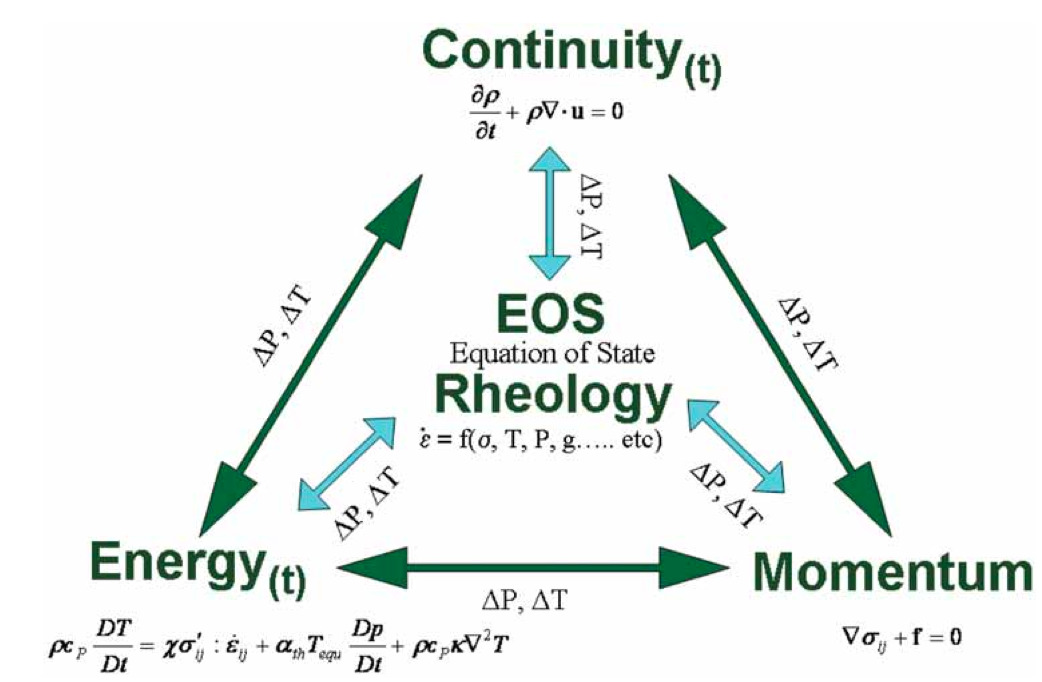
\includegraphics[width=10cm]{images/gravity/reg}\\
{\captionfont
Illustration of the central roles that pressure, temperature and density play in geophysics.\\ 
Taken from Regenauer-Lieb \etal, Phil. Mag., 2006 \cite{rehy06}.
}
\end{center}
 
The internal pressure distribution is directly linked with the Earth's 
own internal gravity field and density distribution because
the local pressure gradient equals the local gravity acceleration
times the density (see problem \ref{problem-pressure}).
In Section~\ref{section_Density-gravity-pressure} density, gravity
and pressure are treated together in a consistent way. 

If the internal pressure distribution is known we can relate sharp
transitions in the physical parameters as shown in the PREM model,
illustrated in the following figure 
to phase transitions, solid-solid or solid-liquid, 
in the Earth's deep interior.

\begin{center}
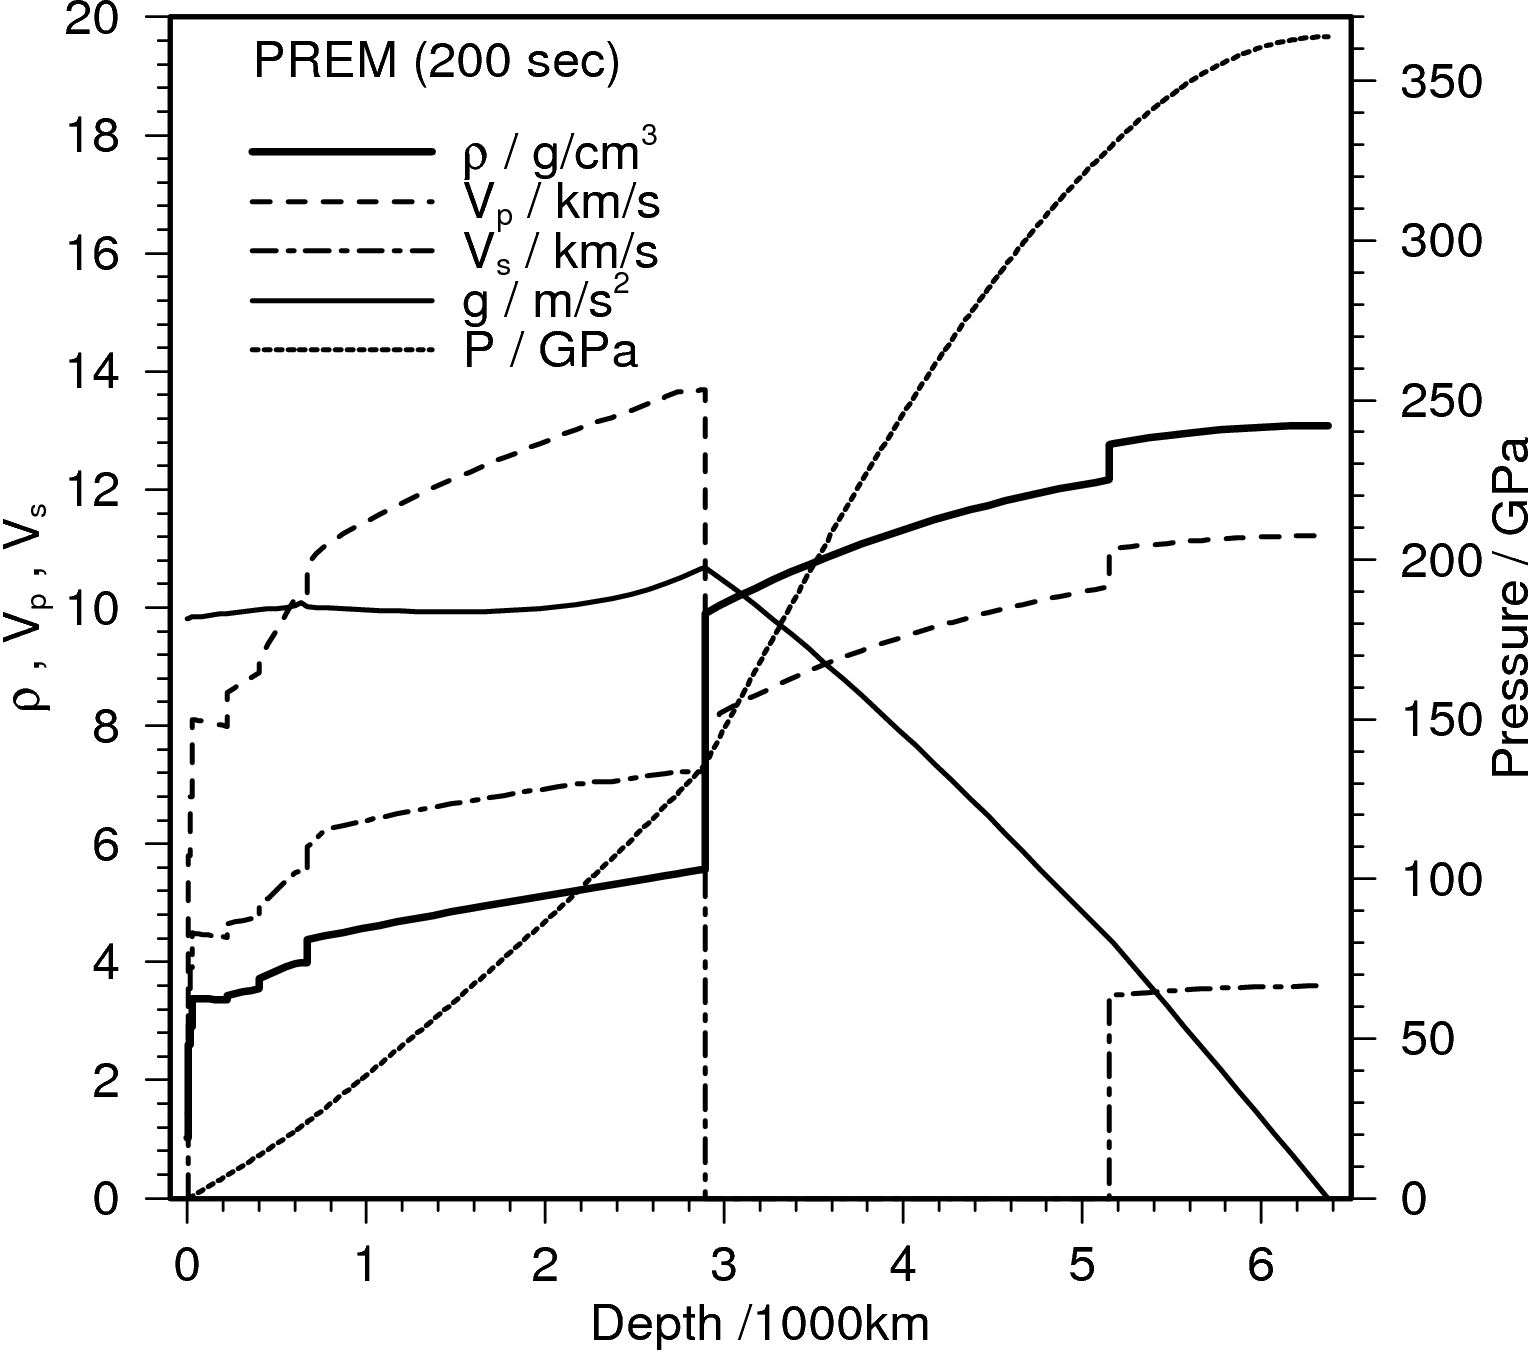
\includegraphics[width=8cm]{images/gravity/PREM-inc-pressure}\\
{\captionfont Radial (depth)distribution of density $\rho$, 
seismic velocities $v_p$ and $v_s$,
gravity acceleration $g$ and pressure $P$ \\
in the PREM model (Dziewonski and Anderson (1981) \cite{dzan81}).}
\end{center}


Phase transitions in `candidate' materials for the Earth's interior
are investigated under high pressure and temperature conditions in
HPT laboratory experiments
\footnote{
Deep Earth pressure and temperature conditions can be produced in 
a Diamond Anvil Cell (DAC),
see \url{http://en.wikipedia.org/wiki/Diamond\_anvil\_cell}.
}.
Using theoretical mineral physics models the complete mineral phase 
diagram of mantle silicates can, in principle,
be constructed from a limited set of experimental data
(Stixrude \& Lithgow-Bertelloni (2005) \cite{stli05,stli05b}
Jacobs \& de Jong (2007) \cite{jade07}).  
To constrain the possible candidate materials we also need to know 
the internal distribution of the Earth's chemical composition.
Such composition models are derived from geological evidence and
cosmochemical considerations.

\index{general}{P.R.E.M.}
Table I of (Dziewonski and Anderson (1981) \cite{dzan81}) gives 
an expression for the density as a function of the radius $r$, which 
I have turned into a python function:
\begin{lstlisting}
def prem_density(radius):
    x=radius/6371.e3
    if radius>6371e3:
       densprem=0
    elif radius<=1221.5e3:
       densprem=13.0885-8.8381*x**2
    elif radius<=3480e3:
       densprem=12.5815-1.2638*x-3.6426*x**2-5.5281*x**3
    elif radius<=3630.e3:
       densprem=7.9565-6.4761*x+5.5283*x**2-3.0807*x**3
    elif radius<=5600.e3:
       densprem=7.9565-6.4761*x+5.5283*x**2-3.0807*x**3
    elif radius<=5701.e3:
       densprem=7.9565-6.4761*x+5.5283*x**2-3.0807*x**3
    elif radius<=5771.e3:
       densprem=5.3197-1.4836*x
    elif radius<=5971.e3:
       densprem=11.2494-8.0298*x
    elif radius<=6151.e3:
       densprem=7.1089-3.8045*x
    elif radius<=6291.e3:
       densprem=2.6910+0.6924*x
    elif radius<=6346.e3:
       densprem=2.6910+0.6924*x
    elif radius<=6356.e3:
       densprem=2.9
    elif radius<=6368.e3:
       densprem=2.6
    else:
       densprem=1.020
    return densprem*1000
\end{lstlisting}

\begin{center}
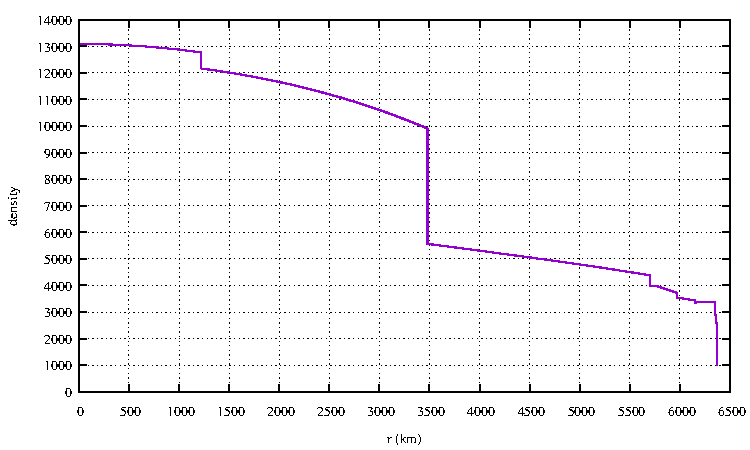
\includegraphics[width=8cm]{images/prem/rho.pdf}
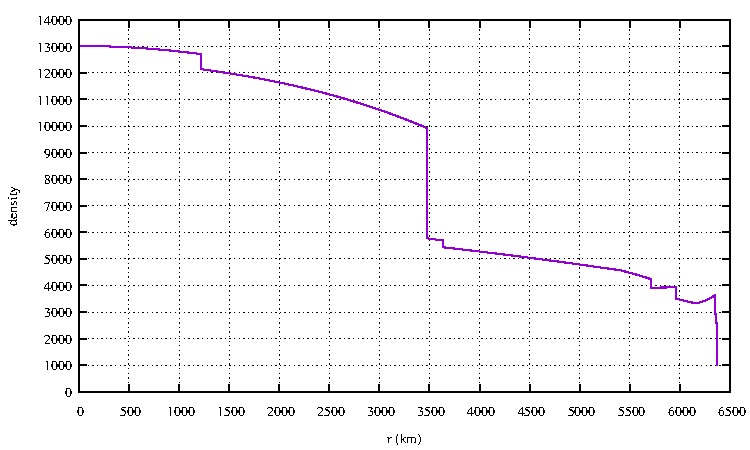
\includegraphics[width=8cm]{images/ak135/rho.pdf}\\
{\captionfont Top: PREM density as computed with the function above. 
Code available in /images/prem/; \\
Bottom: ak135 density from \cite{keeb95}.
Data available in /images/ak135/ } 
\end{center}


%--------------------------------------------------

%--------------------------------------------------
\subsubsection{Early models of the Earth's density}

The total Earth mass $M_{\oplus}$ and average density $\left <\rho \right >$
were not known 
before independent measurement of Newton's gravitational 
constant by Cavendish, 
(see Section~\ref{section_Density-gravity-pressure}).
When the average density had been determined as approximately 
$5.5 \cdot 10^3~\mathrm{kg\cdot m}^{-3}$ it became clear, 
from the lower density of surface rocks of around 
$2.7 \cdot 10^3~\mathrm{kg\cdot m}^{-3}$,
that the Earth's interior must consist of higher density material.

Besides the mass or average density the (average) 
moment of inertia $I$ (defined in Section~\ref{sect_scalarmomint}) 
provides a constraint on the radial distribution of density.
     
These two integral parameter values have been applied in several 
two-parameter models for the radial density distribution of the Earth.
At the end of the nineteenth century Wiechert\footnote{Emil Johann 
Wiechert (26 December 1861 - 19 March 1928) was a German physicist 
and geophysicist who made many contributions to both fields, 
including presenting the first verifiable model of a layered structure of the 
Earth and being among the first to discover the electron.} assumed that the 
compressibility of Earth materials would be negligible to first
approximation and that Earth's high mean density was due to a dense,
probably metallic, core.
He assumed an iron core based on astronomical evidence of high iron
content of the sun's outer layers 
(see also Section~\ref{section-chemical-composition}).

Wiechert considered in particular layered spherically symmetric 
models consisting of two uniform layers, core and mantle.
Since the radius of the Earth's core had not yet been determined by
seismology, Wiechert used the core radius $R_c$ and density 
$\rho_c$ as unknown parameters to be determined from the
known data.
Wiechert assumed the density of the mantle to be 
$\rho_m=3.2 \cdot~10^3 \mathrm{kg\cdot m}^{-3}$ and using known values for $M$ and $I$
he derived for the radius of the core
$R_c/R = 0.779$ corresponding to a mantle depth of about
$1400~\mathrm{km}$ and a core density 
$\rho_c=8.2\cdot 10^3~\mathrm{kg\cdot m}^{-3}$.
This model is investigated in problem 
\ref{problem-wiechert-2layermodel}.

Later, after $R_c/R = 0.545$ had been determined using
seismic data, Jeffreys substituted the known value of the
core radius and derived for the mantle and core densities
$\rho_c=12.6\cdot 10^3~ \mathrm{kg\cdot m}^{-3}$ and 
$\rho_m=4.14\cdot 10^3~ \mathrm{kg\cdot m}^{-3}$ (Bullen (1975) \cite{bull75}).
This model is investigated in problem 
\ref{problem-jeffreys-2layermodel}.

The (radially averaged) density distribution in the Earth remains a topic of research
\cite{kenn98}.
